\documentclass[letterpaper,12pt]{article}

\usepackage{threeparttable}
\usepackage{geometry}
\geometry{letterpaper,tmargin=1in,bmargin=1in,lmargin=1.25in,rmargin=1.25in}
\usepackage[format=hang,font=normalsize]{caption}
\usepackage{amsmath}
\usepackage{mathrsfs}
\usepackage{multirow}
\usepackage{array}
\usepackage{delarray}
\usepackage{amssymb}
\usepackage{amsthm}
\usepackage{lscape}
\usepackage{natbib}
\usepackage{setspace}
\usepackage{float,color}
\usepackage[pdftex]{graphicx}
\usepackage{pdfsync}
\usepackage{verbatim}
\usepackage{placeins}
\usepackage{geometry}
\usepackage{pdflscape}
\synctex=1
\usepackage{bm}
\theoremstyle{definition}
\newtheorem{theorem}{Theorem}
\newtheorem{acknowledgement}[theorem]{Acknowledgement}
\newtheorem{algorithm}[theorem]{Algorithm}
\newtheorem{axiom}[theorem]{Axiom}
\newtheorem{case}[theorem]{Case}
\newtheorem{claim}[theorem]{Claim}
\newtheorem{conclusion}[theorem]{Conclusion}
\newtheorem{condition}[theorem]{Condition}
\newtheorem{conjecture}[theorem]{Conjecture}
\newtheorem{corollary}[theorem]{Corollary}
\newtheorem{criterion}[theorem]{Criterion}
\newtheorem{definition}{Definition} % Number definitions on their own
\newtheorem{derivation}{Derivation} % Number derivations on their own
\newtheorem{example}[theorem]{Example}
\newtheorem{exercise}[theorem]{Exercise}
\newtheorem{lemma}[theorem]{Lemma}
\newtheorem{notation}[theorem]{Notation}
\newtheorem{problem}[theorem]{Problem}
\newtheorem{proposition}{Proposition} % Number propositions on their own
\newtheorem{remark}[theorem]{Remark}
\newtheorem{solution}[theorem]{Solution}
\newtheorem{summary}[theorem]{Summary}
\bibliographystyle{aer}
\newcommand\ve{\varepsilon}
\renewcommand\theenumi{\roman{enumi}}
\newcommand\norm[1]{\left\lVert#1\right\rVert}
\usepackage{dcolumn}
\usepackage{booktabs}
\captionsetup{skip=0.333\baselineskip}
\newcolumntype{d}[1]{D{.}{.}{#1}}
\newcommand\mc[1]{\multicolumn{1}{@{}c@{}}{#1}}
\usepackage[format=plain,
            font=it]{caption}

\begin{document}

\title{Endogenous Heterogeneous Innovation}

\author{Julio Roll\\Scott Behmer\\
  The University of Chicago}

\date{}              % No date for final submission

% Create title page with no page number

\renewcommand{\thefootnote}{\fnsymbol{footnote}}

\singlespacing

\maketitle

\vspace{-.2in}
\begin{abstract}
\noindent 
In this paper, a subset of parameters are estimated for a novel endogenous growth model. Building on previous work in which a distinction is made between different types of innovation, in this model firms choose endogenously between investing in abrupt or incremental innovations. This can lead to many interesting predictions regarding variation in R\&D investment choices over time. The model is fit to citation distributions for the entire US economy using structural estimation methods. The parameter estimates imply that there are no diminishing returns to incremental innovations, which has important theoretical implications.
\end{abstract}

\medskip
\noindent \textit{Keywords}: Endogenous Growth, Innovation, Research and Development, Patents, Citations, Productivity.

\thispagestyle{empty}

\onehalfspacing
\setcounter{footnote}{1}
\renewcommand{\thefootnote}{\arabic{footnote}}
\setcounter{page}{1}

\section{Introduction}

This paper investigates the interpemporal productivity choice that a firm has to make when deciding whether to make incremental or abrupt product innovations. Technological innovation has long been viewed as the main driver of economic growth. It is clear that innovativeness comes in many different types, including in their scale, scope, and type of impact. Recent literature on endogenous growth has included heterogeneity in innovation. In this paper, a model is presented in which firms endogenously choose between two different types of innovation: abrupt (major) and incremental (minor). This feature allows the model to explain a larger range of behavior, and has a number of interesting predictions. In this work, we take a first step toward applying the model; a few key parameters are estimated using data on patent citation distributions.

Our analysis is linked to the literature on endogenous growth, where creative destruction by firms is the main driver of growth. In this sense, firms engage in R\&D both to increase their mark-up and to steal the products of other firms. Although the recent literature on this subject has taken into account the idea of R\&D heterogeneity (Akcigit and Kerr, 2016) and diminishing returns of incremental innovation (Acemoglu, Akcigit and Celik, 2014), innovation is always good for productivity, even in the short-term. Moreover, since the focus of Acemoglu et al. (2014) was in the relationship between management and R\&D, they do not endogenize the innovation decision. Additionally, to our knowledge, there is no model that accounts for the possibility of firms innovating abruptly internally, which ignores the temporal dimension of the decision to innovate.

Under certain parameter values, our model has interesting predictions regarding intertemporal productivity choices by innovating firms. This interesting behavior arises when abrupt innovations result in a relatively small or even negative productivity change. In this case, right after a radical innovation, firms want to benefit from all the possible new incremental innovation steps that they can make. Eventually they exhaust the realm of incremental ideas, so firms turn to abrupt innovation, even though that may result in a temporary decrease in productivity. This cyclical firm behavior would  have important aggregate implications. At any given point, some share of firms will be trading current productivity for future productivity as they choose to engage in abrupt R\&D. However, this productivity decline, which should impact the aggregate measure of TFP in the economy, is not related with sluggish efficiency. It is simply the result of an arbitrage decision that would, ideally, pay off in the future.

Before applying the model to intertemporal productivity decisions, however, we must first estimate a few key model parameters using steady-state patent citation data. Many previous papers have used patent and patent citation data to discipline productivity in an endogenous framework (e.g. Griliches, 1990). The idea behind this identification is that a patent with more citations has a bigger impact on productivity. Using the rich citation distribution available from the empirical work of Hall, Jaffe and Trajtenberg (2001), we discipline our parameters by imposing patent and citation patterns and quantify the impact of each possible innovation path. 

Model parameters are estimated using maximum likelihood estimation and, as a robustness check, the generalized method of moments. Their robustness is also tested to changes in various theoretical assumptions. Our resulting estimates for average arrival rates of both abrupt and incremental innovations are what we would expect given our theoretical model, and they match well with untargeted moments. However, our estimate of another key model parameter is very unexpected. This estimate indicates that incremental innovations are not subject to diminishing returns, which is a key feature of both our model and those from previous papers. If true, this result precludes many of the interesting behavioral predictions of our model, including the intertemporal TFP choice mentioned above. Considering the importance of this result, we devote a large portion of the paper to investigate the theoretical assumptions and empirical features that are driving it.

The paper is structured as follows: section \ref{sec:Data} specifies the databases that were used to estimate the parameters and presents some motivating stylized facts. Section \ref{sec:Model} lays down the theoretical framework used to highlight the R\&D decisions of firms. Section \ref{sec:Estimation} describes the estimation procedure. Section \ref{sec:Results} presents the estimation results and \ref{sec:Conclusion} concludes.

\section{Databases and Motivating Data}\label{sec:Data}

This section provides an overview of the databases that were used in the estimation, as well as some motivating firm-level observations that the theoretical framework proposed in section \ref{sec:Model} will highlight.

\subsection{Databases}

In order to analyze the intrinsic relationship between firm dynamics and R\&D behavior through the lens of patent and citation patterns, we will make use of two databases:

\begin{itemize}
	\item \textbf{NBER-USPTO Patent Database:} Data on patents and citations come from the massive effort undertaken by Hall et al. (2001) in order to count citations of patents granted between 1976-2006. The database has over 3 million patents from the United States Patent and Trademark Office (USPTO), including assignee identification, patent class and citation data. We will limit ourselves to patents granted to US assignees. Moreover, regarding citations, we will use the diffusive correction coefficients from Hall et al. (2001) to adjust for the cutoff effect: as patent applications get closer to the 2006 cutoff, the citation count is, naturally, lower, simply because it did not have enough time to receive citations. The data can also be dynamically matched to the Compustat database;
	\item \textbf{Compustat North American Fundamentals:} Compustat is a database of financial, statistical and market information on active and inactive companies. The database has information over the period 1950-2015 on the US economy. Since privately held firms do not have to disclose financial statements, the database has only publicly-listed firms. However, because those firms tend to be bigger than private ones, they have a significant weight in the whole economy. The main variables are SIC code, employment, net income, net sales, cost of goods sold (COGS), R\&D expenditure, plant, property and equipment and total assets. When price deflators are needed, we use the NIPA tables. Moreover, we remove from the data heavily regulated sectors (e.g. utilities), financial firms and observations in which a firm has made acquisitions larger than 5\% of the value of their total assets.
\end{itemize}

\subsection{Empirical Observations}

The idea of analyzing the intertemporal productivity choice that firms face when deciding whether to continue on the diminishing returns path of incremental innovations or to successfully innovate a product line abruptly, at the expense of a temporary productivity slump, comes from two observations in the data. Even though those observations are not directly related to the estimation procedure in this paper (c.f. section \ref{sec:Estimation}), we deem it important to always have them in mind throughout the analysis.

First, one should note that, since the 1970s (but more strongly in the 1980s), there has been a surge in the number of what we will denote as \textit{"sprinter firms"}: firms that report negative profits, but grow faster than their entire sector of activity (e.g. Amazon in the early 2000s). Figure \ref{fig:CBFirms} highlights the increasing share of sprinter firms in the US economy. This fact is robust if, instead, we weight each company by their employment share. Impressive in itself, this observation is doubly interesting by the fact that those firms invest more in R\&D, when comparing median values, than the entire economy. Figure \ref{fig:RD_spending_rat} shows the evolution of this ratio for the US economy. This observation is robust if we restrict comparisons by SIC Code.

If we assume that firms, at some point, should start making profits, this means that a significant share of firms are entering in a temporary R\&D "sprint race": they increase their innovation effort in order to succeed. The theoretical framework behind this rationale is that, after making an abrupt innovation, a firm is impacted by a productivity decline. However, since a radical innovation opens a new production potential, returns to R\&D are bigger, hence companies have an incentive to make R\&D efforts.

Secondly, the productivity slump from abrupt innovation is observed at the firm level. Table \ref{tab:Pat_reg} shows a persistent and significant labor productivity decline 4 years after a firm files an abrupt patent application (taken, here, as the top 10\% of patents in number of citations). This is done by regressing firm-level labor productivity growth with lagged dummy variables that capture the (lagged) arrival of an abrupt patent. We also control for firm-level fixed effects and yearly fixed effects that could be related with macro technological shifts. This goes in line with the idea that those type of patents require a major shift in production (e.g. labor, machines), imposing a productivity toll since firms have to rebuild their accumulated knowledge in the new production (at the momentary expense of profits).

In section \ref{sec:Model}, we propose a model that will highlight the R\&D pattern observed in both of these stylized facts through the complementary dynamic between incremental and radical innovations.

\section{The Model} \label{sec:Model}

The baseline theoretical framework used here is similar to the one employed in Ackigit and Kerr (2016) and Acemoglu et al. (2014). A firm is defined as a portfolio of product lines $\mathscr{F}_j$ as in Klette and Kortum (2004) and can engage in both internal and external R\&D. Differently from the previous literature, the goal here is to highlight each firms' choice of investing in incremental R\&D, subject to diminishing returns, and internal abrupt innovation, which causes a temporary productivity slump, along the quality ladder of a product. As a simplification, R\&D does not scale with firm size.

Because the estimation concerns only the innovation effort of firms, we will limit ourselves to the partial equilibrium.

\subsection{Production}

We consider a continuous-time setup where preferences are determined over a unique final good $Y(t)$, produced by labor and a continuum of intermediate goods $j \in [0,1]$ with the CES production technology defined by:

\begin{equation} \label{eq:Prod}
Y(t) =  \frac{L^{\beta}}{1 - \beta}\int_0^1 q_j^{\beta}(t)k_j^{1-\beta}(t)dj
\end{equation}

\noindent where $q_j(t)$ is the productivity of product $j$, $k_j$ its quantity and $L$ is the production labor supply, which is supplied inelastically. 

Since each product line owned by a firm is independent of the others, prices are set in order to maximize profits in each line. Each patent allows for monopoly pricing in each product line by the leading-edge firm, which faces a constant marginal cost $\zeta$. As a simplification, when there is an abrupt innovation, we will assume that the production of the old generation variety is shut-down, being replaced by the new version, even in the presence of a productivity decline.

As such, according to~\eqref{eq:Prod}, firms face, for each $j$, an iso-elastic inverse demand defined as (time arguments were suppressed for clarity):

\begin{equation} \label{eq:Price}
p_j =  L^{\beta}q_j^{\beta}k_j^{-\beta}
\end{equation}

The profit-maximization problem, then, can be written as:

\begin{equation} \label{eq:PiMax}
\Pi(q_j) = \max\limits_{k_j \geq 0}\Big\{L^{\beta}q_j^{\beta}k_j^{1-\beta} - \zeta k_j\Big\}
\end{equation}

The first-order condition for~\ref{eq:PiMax} yields, for each intermediate good $j$:

\begin{equation} \label{eq:FOC}
p_j = \frac{\zeta}{1-\beta}\; \texttt{and}\;k_j = \Big[\frac{1-\beta}{\zeta}\Big]^{\frac{1}{\beta}}Lq_j
\end{equation}

Hence, equilibrium profits for each product line are linear in quality $q_j$:

\begin{equation} \label{eq:EqProfit}
\Pi(q_j) = \beta\Big[\frac{1-\beta}{\zeta}\Big]^{\frac{1-\beta}{\beta}}Lq_j \equiv \pi q_j
\end{equation}

\subsection{Research and Development Dynamics}

Firms have profit-incentives to innovate in their own product lines through \textit{internal innovation}, thus increasing productivity. Moreover, firms have incentives to do abrupt innovation on other the products of other firms, "stealing" the product line of another firm by developing a new product generation through \textit{external innovation}. For internal R\&D, firms can invest in \textit{incremental innovation}, thus increasing, with diminishing returns, the productivity of the current product generation, and in \textit{internal abrupt innovation}, "killing" the current generation and resetting the cycle for returns of incremental innovation (meaning a new generation can achieve higher productivity levels) at the expense of reducing its current productivity. Here, differently from other models, the process of creative destruction is limited to the development of a new product generation over the current version belonging to another firm. The entire process is determined endogenously. 

This R\&D dynamic is summarized in figure \ref{fig:QLadder} and will now be described in detail.\\

\textbf{Incremental R\&D:} Firms can improve their current product $j \in \mathscr{F}_j$, within their current technological generation (e.g. from an iPhone 3G to an iPhone 3GS), by investing $C_{inc,k}$ units of the final good at each innovative step $k \geq 0$. This cost is defined as:

\begin{equation} \label{eq:Cinc}
C_{inc,k}(\lambda_{inc,k},q_j) = \xi_{inc}\lambda_{inc,k}^{\psi_{inc}}q_j
\end{equation}

\noindent where $\lambda_{inc,k} \ge 0$ is the desired incremental innovation instantaneous Poisson flow rate for each level $k$, $\xi_{inc}$ is the incremental R\&D scale and $\psi_{inc}$ is the elasticity of innovation effort to R\&D expenditures. When successful, the productivity improves such that $q(t + \Delta t) = q(t)(1 + \sigma\alpha^{k})$, where $\sigma > 0$ is a constant multiplicative step-size, $\alpha \in [0, 1]$ is the decay rate of doing sequential incremental steps.\\

\textbf{Internal Abrupt R\&D:} Firms can also improve a product by making a generational step (e.g. from an iPhone 3GS to the iPhone 4). In that sense, they spend $C_{int, abr}$ units of the final good, defined as:

\begin{equation} \label{eq:Cintabr}
C_{int,abr}(\lambda_{int,abr},q_j) = \xi_{abr}\lambda_{int,abr}^{\psi_{abr}}q_j
\end{equation}

\noindent where $\lambda_{int,abr} \ge 0$ is the internal abrupt innovation instantaneous Poisson flow rate, $\xi_{abr}$ is the abrupt R\&D scale and $\psi_{abr}$ is the elasticity of innovation effort to R\&D expenditures. When successful, the productivity improves such that $q(t + \Delta t) = q(t)\gamma_{int,abr}$, where $\gamma_{int,abr} \in [0,1]$ is the productivity slump required for a generational evolution.\\

\textbf{External R\&D:} Finally, firms can engage in creative destruction by innovating (abruptly) on the product line of other firms. This is done by investing $C_{ext}$, defined as:

\begin{equation} \label{eq:Cext}
C_{ext}(\lambda_{ext},\bar{q}_j) = \xi_{abr}\lambda_{ext}^{\psi_{abr}}\bar{q}_j
\end{equation}

\noindent where $\lambda_{ext} \ge 0$ is the instantaneous Poisson flow rate for external R\&D and $\bar{q}_j$ is the average productivity in the whole economy. Similar to the internal innovation effort, the subsequent productivity is given by $q(t + \Delta t) = \bar{q}(t)\gamma_{ext}$, $\gamma_{ext} \in [0,1]$. In this case, the product line joins the portfolio of the innovating firm and the firm losing its product may exit the market if its portfolio is empty.\\

\textbf{Patent and Citation Behavior:} The proposed innovation dynamic assumes a structure of patent and citation arrival. Firms can move vertically and horizontally in the quality ladder of each product by creating patents. Each generation of a product is owned by a single firm, who owns the original abrupt patent and can innovate over it incrementally. Latter incremental patents are assumed to cite all previous patents within a generation. Finally, the cycle is rewound when that same firm makes an internal abrupt innovation or when other firms or entrants innovate abruptly on that product line. This pattern implies that abrupt patents receive more citations.

\subsection{Entrants}

Similar to Klette and Kortum (2004), a mass of entrants engage in R\&D in order to enter the economy by successfully innovating abruptly on a product line. Entrant R\&D cost $C_e$ is defined as:

\begin{equation} \label{eq:Ce}
C_e(\lambda_e,\bar{q}_j) = \nu\lambda_e\bar{q}_j
\end{equation}

\noindent where $\lambda_e \ge 0$ is the innovation flow rate and $\nu \ge 0$ is a scale parameter. As such, the value $V_0$ of being an entrepreneur can be written as the expectation of successfully innovating:

\begin{equation} \label{eq:V0}
rV_0 - \dot{V} = \max\limits_{\lambda_e}\big\{\lambda_e\big[E_jV(\{\bar{q}_j\gamma_{ext},0\}) - V_0\big] - C_e\big\}
\end{equation}

\noindent where $r$ is the interest rate, $V(q_j)$ is the value of owning one product with productivity $q_j$ and $\dot{V}$ is the partial derivative with respect to time.

Free-entry condition requires that:

\begin{equation} \label{eq:Free-entry}
E_jV(\{\bar{q}_j\gamma_{ext},0\}) = \nu\bar{q}_j
\end{equation}

Hence, all product lines are subject to an aggregate rate of creative destruction $\tau$ from all $n_f$ firms in the economy and the outside entrants, where:

\begin{equation} \label{eq:Tau}
\tau = n_f\lambda_{ext} + \lambda_e
\end{equation}

\subsection{Incumbents}

The incumbents value function determines the amount of R\&D effort. Given a product portfolio with $n_p$ products, a vector of productivities $\overrightarrow{q}_f \equiv \{q_{f,j_1}, q_{f,j_2}, ..., q_{f,j_{n_p}}\}$ and a vector of the number of incremental steps $\overrightarrow{k}_f \equiv \{k_{f,j_1}, k_{f,j_2}, ..., k_{f,j_{n_p}}\}$, a firm chooses each innovation flow rate so as to maximize:

$rV(\{q_t,k\}) - \dot{V}(\{q_t,k\}) =$
\begin{equation} \label{eq:Vincumb}
\max_{\substack{\lambda_{inc,k}\\\lambda_{int, abr}\\\lambda_{ext}}}\left[\begin{aligned}
		&\sum_p^{n_p}\left[\begin{aligned}
			&\qquad\qquad\quad\pi n_{p} - \xi_{inc}\lambda_{inc,k}^{\psi_{inc}}q_t - \xi_{abr}\bar{q}_t\lambda_{int,abr}^{\psi_{abr}}\\
			& + \lambda_{inc,k}\big[V(\{q_t^{p-}, k^{p-}\}\cup \{q_{t+\Delta t, j_p}, k_{j_p} + 1\}) - V(q_{t},k)\big]\\
			&+ \lambda_{int, abr}\big[E_j\big[V(\{q_t^{p-},k^{p-}\}\cup \{q_{t+\Delta t,j_p}, 0\}\big] - V(q_{t},k)\big]\\
			&\qquad\quad \ \ - \tau\big[V(\{q_t,k\}\setminus \{q_t^p,k^p\}) - V(q_t,k)\big]\\
		\end{aligned}\right]\\
		&+ \lambda_{ext, abr}\big[E_j\big[V(\{q_t,k\}\cup \{q_{t+\Delta t}^{p'},0\}\big] - V(\{q_t,k\})\big] - \xi_{abr}\bar{q}_t\lambda_{ext}^{\psi_{abr}}
	\end{aligned}\right] 
\end{equation}

The right-hand side of the value function is quite intuitive: the first four lines are common to all product lines owned by a firm. The first line represents the instant returns minus the R\&D costs of doing incremental and abrupt internal innovation. The second line has the expected return flows from doing incremental innovation on product $p$, whose productivity changes with the single incremental jump. Similarly, the third line describes the return flows of doing internal abrupt R\&D. In this case, the productivity change comes with a reset of the number of incremental steps. Lastly for each product line, the forth line represents the effect of creative destruction by another firm, when the incumbent loses one of its products. Equivalently, the last line is due to the fact that firms can also engage in external abrupt innovation themselves, in which case it adds one product to its portfolio by investing in external R\&D.

Since the focus of this paper is on the estimation of the citation distribution and the innovation-related parameters, we will refrain from proposing a solution to the value function here.

\subsection{Stationary Distributions of Products and Citations}

At the steady state, the economy has a stationary distribution of products at each incremental step. Since abrupt patents are cited by all the subsequent incremental ones within each generation of a product, the citation distribution of abrupt patents and the stationary distribution of products follow the same pattern. We will describe the former now.

Denote $\eta_k$ the share of abrupt patents that have received $k$ citations (which is equivalent of having $k$ incremental arrivals). For each $k$ in all product lines (which we normalize to measure 1), at the steady state, we must have outflows balancing inflows, i.e.:

$$\begin{array}{llll}
\textit{Level} & \textit{Inflow} &  & \textit{Outflow}\\
k = 0 & \tau + \lambda_{int,abr} & = & \eta_0(\lambda_{inc,0} + \lambda_{int,abr} + \tau)\\
k \geq 1 & \eta_{k-1}\lambda_{inc,k-1} & = & \eta_k(\lambda_{inc,k} + \lambda_{int,abr} + \tau)\\
\end{array}$$

For the first citation level, inflows come from the aggregate arrival of internal abrupt patents from all steps and from external creative destruction, while outflows originate from products at level 0 that get an incremental innovation (i.e. a new citation), from internal abrupt innovation of product lines with no citation and from creative destruction. For all the other citation levels $k$, inflows come from successful incremental R\&D from the previous level $k-1$, while outflows are either a result of patents with $k$ citations receiving a citation from a subsequent incremental development, from abrupt internal innovation at that level or from outside creative destruction.

Solving for all levels gives:

\begin{equation} \label{eq:eta0}
\eta_0 = \Big[\frac{\lambda_{int,abr} + \tau}{\lambda_{inc,0} +\lambda_{int,abr} + \tau}\Big]
\end{equation}

\begin{equation} \label{eq:etak}
\eta_k = \eta_{k-1}\Big[\frac{\lambda_{inc,k-1}}{\lambda_{inc,k} +\lambda_{int,abr} + \tau}\Big]
\end{equation}

\section{Estimation}\label{sec:Estimation}

In this section, we will describe the estimation procedure that was employed in order to estimate the model parameters that are related to R\&D. This is done by taking the model predictions directly to the USPTO data on patents and citations. Even though we do not estimate the model in its entirety, the innovation-related parameters are the core of the theoretical framework.

\subsection{Link Between Patent Citations and Theory}
Multiple assumptions are needed to relate the various features of the patent citation dataset to our theoretical model:
\begin{itemize}
	\item i) Every patent represents a single innovation;
	\item ii) Abrupt patents will receive more total citations than incremental patents;
	\item iii) An abrupt patent receives a citation from a patent within its same classification if and only if the citing patent represents an incremental innovation within the abrupt patent’s technology cluster;
	\item iv) Internal innovations will receive more self-citations (citations from future patents by that same company) than external innovations.
\end{itemize}
Assumptions \textit{i}, \textit{ii}, and \textbf{iv} are made in Akcigit and Kerr (2016) based on empirical evidence (albeit of varying degrees). Assumption \textit{iii} is very important to our estimation scheme and a natural one to make. It states that every incremental innovation will cite the abrupt patent that started its technology cluster, and that they will always be within the same patent classification. This provides a clear link between the data and the theoretical distribution in equations \ref{eq:eta0} and \ref{eq:etak}. If the technology cluster of an abrupt innovation had k incremental innovations, the related patent will receive k same-class citations.

Of course, in order to estimate the model we also need to identify the abrupt patents. Assumption \textit{ii} states that abrupt patents will have more total citations (same-class plus external-class citations), but it does not give us an exact cutoff. In Akcigit and Kerr (2016), they estimate that the upper 10\% of the total citation distribution contains the abrupt patents, so we use this cutoff in our baseline estimation. Later we test the robustness of our estimates to changes in this value.

Using the 10\% cutoff, we can generate the distribution of same-class citations to abrupt patents (c.f. figure \ref{fig:SameClassDistr}). This empirical distribution will be fit to our theoretical distribution from equations \ref{eq:eta0} and \ref{eq:etak} to estimate the model. Two important features of the empirical distribution are the large mass of patents at zero citations and the large upper tail.

It should be noted that, even if the four assumptions listed above are completely accurate, we would expect some abrupt patents to be wrongly classified as incremental due to our 10\% cutoff. According to our theoretical model, there is a chance that the technology cluster of an abrupt will be replaced very early on by another abrupt innovation, meaning that it will receive very few same-class citations. While the abrupt patent could still receive out of class citations after being replaced (and in fact, we do see many patents with zero same-class citations but many external citations), it could not receive enough to be classified as abrupt. Thus, we expect the empirical distribution in figure \ref{fig:SameClassDistr} to underestimate the amount of abrupt patents with low numbers of citations. The impact of this potential bias on our estimation is discussed below.

\subsection{Maximum Likelihood Estimation}

According to equations \ref{eq:eta0} and \ref{eq:etak}, the theoretical citation distribution of abrupt patents only depends on three parameters: $\alpha$, $\lambda_{inc,0}$, and $\lambda_{abr, int} + \tau$. In addition, the distribution is identical at equal ratios of the arrival rate parameters, so it actually only depends on two independent parameters: $\alpha$ and $\frac{\lambda_{abr, int} + \tau}{\lambda_{inc,0}}$. Intuitively, $\alpha$ governs rate at which the incremental innovation step size decays after multiple incremental innovations ($\alpha$ equal to one implies a constant step size). The value of $\frac{\lambda_{abr, int} + \tau}{\lambda_{inc,0}}$ is determined by the relative amount of incremental compared with abrupt innovations in the entire economy.

Given a set of parameter values, the resulting citation distribution looks like a gamma distribution, with a large upper tail and the possibility of a mode greater than zero. A larger value of $\frac{\lambda_{abr, int} + \tau}{\lambda_{inc,0}}$  means that there are relatively more abrupt innovations, which means that more product lines will be replaced before their originating patents can accrue a large number of citations. Thus, increasing $\frac{\lambda_{abr, int} + \tau}{\lambda_{inc,0}}$ shifts the distribution to the left. Reducing the value of $\alpha$ means that the firms will invest relatively more in incremental innovation early in the product life-cycle (due to the diminishing returns to incremental innovation). For low enough values of $\alpha$, this can lead to a peak in the distribution at a citation value greater than zero, as firms almost always invest in the first incremental innovation but invest increasingly less in the late ones. Theoretical graphs for various parameter values are shown in figure \ref{fig:ImpactPar}.

We estimate the two parameters using a Maximum Likelihood Estimation (MLE). Our theoretical model gives a probability mass distribution for every whole number of citations, but the actual data shows fractional values (this is due to the diffusive correction factor from Hall et al., 2001). To address this, we rounded the expected citation variable to the nearest whole number, and then took the likelihood as the theoretical PMF value at that point.

The resulting parameter estimates are shown in table \ref{tab:MLETable}, and the fit is plotted in figure \ref{fig:MLE}. The estimated ratio of incremental to abrupt patents is about 10:1, which is consistent with the fact that we defined the upper 10\% of patents in the citation distribution as being abrupt. The estimate of $\alpha$ is equal to one. This indicates that firms do not face diminishing returns to initial investment. This has very important theoretical implications, which will be discussed later on.

\begin{table}[htbp]\centering \captionsetup{width=5.8in}
    \caption{\label{tab:MLETable}\textit{Results from the maximum likelihood estimation}}
	\centering
	\begin{tabular}{>{\small}l >{\small}l >{\small}c >{\small}r}
	\toprule
	Parameters & \multicolumn{1}{c}{$\alpha$} & \multicolumn{1}{c}{$\frac{\lambda_{abr, int} + \tau}{\lambda_{inc,0}}$} & \multicolumn{1}{c}{Criterion}\\
	\midrule
	Results & 1.0 & 0.0995 & 634983.15\\
	\bottomrule
	\end{tabular}
\end{table}

Looking at figure \ref{fig:MLE}, we see that the data fits most of the distribution closely (including the upper-tail, which is not pictured), but significantly underestimates the amount of zero-citation patents. We find that, when observations in the upper tail are eliminated, the estimation better fits the zero-citation data (see figure \ref{fig:MLE_extail}), indicating that the model is unable to completely capture both of those features. Now, it may seem fairly ad-hoc to eliminate observations in the upper tail, but there may be a theoretical justification for doing so. Our model, in keeping with Akcigit and Kerr (2016), only allows for two scales of innovation: abrupt and incremental. This assumption, while it allows for some mathematical simplicity, is clearly a simplification of reality. While there is plenty of evidence that some patents are more valuable than others, there seems to be no evidence of a binary distinction. One might expect that patents in the upper tail of our empirical distribution (it had a max of 741 citations) are significantly more productive than the others. However, under our binary model, those patents are identical to the others from a productivity standpoint, and the only reason they gained more citations was through chance. Thus, because a more complete model may place the upper-tail observations in a separate classification, it is reasonable to be suspicious of estimation results that are pinned down by the upper-tail.

Multiple methods were used to make sure that the parameter values given in figure \ref{fig:MLE} were in fact those that maximize the log-likelihood function. First, many initial values were used in the optimization algorithm, and it always gave the same result. We also tried fixing the value of $\alpha$ and running an unconstrained optimization to determine $\frac{\lambda_{abr, int} + \tau}{\lambda_{inc,0}}$, and this also gave the same result (the motivation being that the unconstrained algorithm is sometimes less sensitive to initial conditions). Finally, the 3D plot of the negative log-likelihood clearly shows a minimum at our parameter values (see figure \ref{fig:Crit}), and a basin hopping algorithm found no other minimum.

Recall that our empirical distribution likely underestimates the number of abrupt patents with a low number of citations. This implies that our theoretical model may actually be even worse at fitting the zero-citation density than figure \ref{fig:MLE_extail} would suggest. It also implies that our estimate of $\frac{\lambda_{abr, int} + \tau}{\lambda_{inc,0}}$ may be biased downward. Importantly, however, because lowering $\alpha$ leads to a decrease in the theoretical density at zero, this downward bias is probably not impacting our estimate of $\alpha$; if the bias was corrected, we would still expect $\alpha$ to be equal to one.

\subsection{First Robustness Check: Generalized Method of Moments Estimation}

Before drawing strong conclusions from our estimation, we ran several robustness checks. These were meant to test the sensitivity of our estimates both to changes in the estimation procedure and to changes in theoretical assumptions. We are mainly interested in seeing if $\alpha$ remains equal to one (no diminishing returns to incremental innovations) and if the fit of the model to the data is affected.

First, we re-estimated the parameters using an alternative estimation scheme: Generalized Method of Moments (GMM). The adopted strategy was to estimate $\hat{\theta}_{GMM} = (\tau + \lambda_{int,abr}, \lambda_{inc,0}, \alpha)$ by solving equation~\eqref{eq:GMM} with the actual and the estimated moments ($m^d(x)$ and $m^e(x|\theta_{GMM})$, respectively, where $x$ is the real data).

\begin{equation} \label{eq:GMM}
\mathscr{L}(\theta_{GMM}) =  \min\limits_{\theta_{GMM}}e(x|\theta_{GMM})^TWe(x|\theta_{GMM})
\end{equation}

\noindent where $W$ is the weighting-matrix ($W = I$ here) and $e(x|\theta_{GMM})$ is the moment error function, defined as

\begin{equation} \label{eq:GMM_error}
e(x|\theta_{GMM}) \equiv \frac{m^e(x|\theta_{GMM}) - m^d(x)}{m^d(x)}
\end{equation}

In order to estimate those 3 parameters over the distribution of citations, a set of 4 moments was used: the average number of citations, the average of the first 5 sequential share ratios (e.g. \# of patents with 1 citation/\# of patents with 0 citations), the sum of the first two shares and the incremental R\&D intensity, defined in equation~\eqref{eq:RDintens} similarly to Akcigit and Kerr (2016).

\begin{equation} \label{eq:RDintens}
\texttt{R\&D intensity} = \frac{\beta\xi_{inc}\displaystyle\sum_{k=0}^{\infty}\eta_k\lambda_{inc,k}^2}{share_{inc}\pi}
\end{equation}

\noindent where $\beta = 0.106$ and $\pi = 0.0755$ are calibrated parameters from the general equilibrium and $\xi_{inc} = 0.346$ is the incremental R\&D scale (also calibrated).

Although no single parameter can be singled out with one particular moment, each of the proposed moments has an underlying intuition behind it:

\begin{itemize}
	\item The average number of citations and the R\&D intensity: two global measures of mass that, together, allow for the identification of $(\tau + \lambda_{int,abr})$ and $\lambda_{inc,0}$;
	\item Mean of the initial ratios: given that the initial incremental R\&D effort is a few times bigger than the creative destruction ($(\tau + \lambda_{int,abr})$), one would expect the initial reduction of incremental innovation to be related with the decay parameter $\alpha$;
	\item Sum of the first 2 bins: due to the presence of a significant discontinuity at zero citations (after all, "having ideas" is a highly skewed business), this moment adds an extra weight so as to pin down that effect.
\end{itemize}

The results of the estimation can be seen in Table \ref{GMMTable}. The overall estimation comes fairly close to matching all the data moments, while the estimated parameters are similar to the ones obtained with the MLE. As before, those results are robust to different initial conditions and to a "basin hopping" search. The estimation plot over the data histogram is available in the Appendix.

\begin{table}[htbp] \centering \captionsetup{width=5.8in}
    \caption{\label{GMMTable}\textit{Estimated and data moments using the Generalized Method of Moments}}
	\centering
	\begin{tabular}{>{\small}l >{\small}c >{\small}c}
	\toprule
	Moment & \multicolumn{1}{c}{Data} & \multicolumn{1}{c}				{Model} \\ 
	\midrule
	Mean of citations & 10.06 & 7.39\\
	Mean of first 5 seq. ratios & 0.57 & 0.88\\
	Sum of first 2 bins & 0.26 & 0.22\\
	R\&D Intensity & 0.068 & 0.068\\
	Criterion & & 0.386\\
	\midrule
	$(\hat{\tau} + \hat{\lambda}_{int,abr}, \hat{\lambda}_{inc,0}, \hat{\alpha}) = (0.047, 0.351, 1)$\\
	\bottomrule
	\end{tabular}
\end{table}

To test for robustness on both GMM and MLE, we have also checked the predictions of both models on an untargeted moment: the share of incremental R\&D effort over total effort. Results can be seen in table \ref{Untarg}. Both models presented a close match to the value observed in the data.

\begin{table}[htbp] \centering \captionsetup{width=5.8in}
    \caption{\label{Untarg}\textit{Estimated and actual results for the untargeted share of incremental R\&D effort}}
	\centering
	\begin{tabular}{>{\small}l >{\small}c >{\small}c}
		\toprule
		Moment & \multicolumn{1}{c}{Data} & \multicolumn{1}{c}				{Model} \\ 
		\midrule
		MLE\\
		\;Incremental/total & 0.90 & 0.91\\
		GMM\\
		\;Incremental/total & 0.90 & 0.88\\
		\bottomrule
	\end{tabular}
\end{table}

\subsection{Other Robustness Checks}

The GMM results suggest that the main features of our MLE estimation are not simply artifacts of that specific estimation strategy. Given our theoretical model, the best fit of the data truly seems to be one where the density at zero is underestimated and where alpha is equal to one.

As far as theoretical assumptions, we will now test the robustness of our estimates to variations in the 10\% cutoff that defines an abrupt innovation. While the 10\% value is similar to the one estimated by Akcgit and Kerr (2016) and is used in other papers, those papers use a different theoretical model. Furthermore, there is no defining feature of the citation distribution at the 10\% cutoff (e.g. no discontinuity or anything). Considering this, it is necessary to check whether our results are robust to changes in this cutoff.

The MLE estimates for cutoffs of 20\% and 5\%, alongside the baseline results, are shown in table \ref{tab:Cutoff}. We see that the arrival rates move in the direction that one would expect; the relative amount of abrupt patents drops when the cutoff is 5\% and increases when the cutoff is 20\%. More importantly, we find that $\alpha$ is still equal to one.

\begin{table}[htbp]
	\caption{MLE results for different abrupt cutoff levels.}
	\centering\label{tab:Cutoff}
	\begin{tabular}{>{\small}l >{\small}c >{\small}c >{\small}c}
		\toprule
		Abrupt Cutoff & \multicolumn{1}{c}{10\%} & \multicolumn{1}{c}{5\%} & \multicolumn{1}{c}{20\%}\\ 
		\midrule
		$\lambda_{inc, 0}$ & 0.357 & 0.362 & 0.347 \\
		$(\lambda_{abr} + \tau)$ & 0.0355 & 0.0239 & 0.0568\\
		$\alpha$ & 1.0 & 1.0 & 1.0\\
		\bottomrule
	\end{tabular}
\end{table}

Next we focused on the assumption that an incremental patent will always cite the abrupt patent that initiated its technology cluster. This assumption, which we initially made for mathematical simplicity, is inconsistent with the conclusions of Akcigit and Kerr (2016). In their model, they included a certain probability $p$ that an abrupt patent will be cited by subsequent incremental patents, which was estimated to be 75\%. Adding this parameter to our model is simple. For a technology cluster of size $k$, the probability of the abrupt patent having $i$ citations is given by the binomial distribution:

\begin{equation} \label{eq:prob}
Prob_{i, k} = Binom{i, k, p}
\end{equation}

Thus, given the size distribution $\eta_k$ from equations \ref{eq:eta0} and \ref{eq:etak}, the citation distribution $f_i$ is given by:

\begin{equation} \label{eq:cit_dist}
f_i = \displaystyle\sum_{k=0}^{\infty}\eta_k * Prob_{i, k}
\end{equation}

The addition of the probability parameter $p$ gives the model more flexibility. A lower value of $p$ shifts the distribution left.

The MLE estimates for this updated model are presented in table \ref{tab:Prob}. We see that $p$ is equal to one, with the other parameters identical to our baseline model. This seems to validate our original assumption of setting $p$ equal to one. There are a few caveats, however, with this robustness check. First, as was mentioned above, even in our baseline model there is a problem with the classification of abrupt patents. It is likely that abrupt patents which are displaced early on by another abrupt patent will never gain enough citations to reach our cutoff value. This leads our empirical distribution (shown in figure \ref{fig:SameClassDistr}) to underestimate the number of abrupt patents with a low number of citations. When the probability of citing is less than one, we would expect this underestimation to be even greater. This bias could cause us to overestimate the value of $p$.

\begin{table}[htbp]
	\caption{Robustness Specification Results}
	\centering\label{tab:Prob}
	\begin{tabular}{>{\small}l >{\small}c >{\small}c}
		\toprule
		    & \multicolumn{1}{c}{Baseline} & \multicolumn{1}{c}{Flexible}\\ 
		\midrule
		$\frac{\lambda_{inc, 0}}{(\lambda_{abr} + \tau)}$ & 0.104 & 0.104 \\
		$\alpha$ & 1.0 & 1.0\\
		$p$ & - & 1.0 \\
		log-likelihood & -627597 & -627598 \\
		\bottomrule
	\end{tabular}
\end{table}

While we were able to test the robustness of our estimation to multiple key theoretical assumptions, there are still others that have not been checked. Of these, we think the most in need of support are assumptions \textit{i} and \textit{ii} from the citation section: that abrupt patents will receive a large number of total citations and that same-class citations are those that directly fall within the technology cluster of the abrupt patent. Intuitively, this seems like it may be a good approximation, since one would expect that abrupt innovation embodies important technological breakthroughs, and it is similar to other assumptions made in previous papers. However, we do not have any actual empirical evidence to support it. Considering that our whole estimation strategy rests on those assumptions, further empirical research into their validity is needed.

\section{Results}\label{sec:Results}
%Add a further discussion of the importance of alpha =1 in relation to the broader motivations of the paper (that is, its relations to intertemporal tfp choice).

Through all robustness checks, the most constant result was that $\alpha = 1$. This has very important theoretical implications. If accurate, it indicates that there are no diminishing returns to incremental innovations. This severely limits the strategic behavior predicted by the model. With $\alpha$ less than one, we would expect to see firms cycle between abrupt and incremental R\&D, as incremental innovations are initially very profitable following an abrupt innovation, but eventually dry up. It is this dynamic that led to interesting predictions involving intertemporal productivity choice. With $\alpha$ equal to one, however, the profitability of incremental innovations is completely independent of the timing of the last abrupt innovation. Firms will always invest a constant amount in either type of innovation unless there are changes in the exogenous parameters of the model.

It should be noted that other authors$^1$\footnotetext{Such as Akcigit and Kerr (2016) and Acemoglu et al. (2014)} do not find such a robust constancy of returns on incremental innovation. This could mean that the theoretical framework requires additional complexity (e.g. variable internal abrupt arrival rates).

Our estimates of $\lambda_{abr, int} + \tau$ and $\lambda_{inc,0}$, as expected, are sensitive to theoretical assumptions, especially the assumption that defines abrupt patents as a certain upper percentile of the citation distribution. When we assume that abrupt patents are the upper 10\% of patents, we find the abrupt arrival rate $\lambda_{abr, int} + \tau$ to be between nine and ten times smaller than the incremental arrival rate $\lambda_{inc,0}$. When the cutoff is raised or lowered, the arrival rate parameters move in the direction that one would expect. Now, there was no guarantee that our estimates would match up with our assumptions this well; the patent citation distribution could have been shaped such that our ratio of lambdas was completely different from our assumed fraction of abrupt patents. Thus, these parameter estimates slightly increase our confidence in the model's ability to fit reality.

Regarding innovation dynamics, the fact that incremental R\&D does not run into diminishing returns would discourage firms to do internal abrupt innovation, since the main incentive behind this type of R\&D is that the incremental steps are reset, allowing for a higher potential productivity. If there is no decay, firms can reach such productivity levels just by doing incremental innovation. 

\section{Conclusion}\label{sec:Conclusion}
The estimation presented in this paper is meant to be a first step toward the application of a novel endogenous growth model. The model is an updated version of that developed by Akcigit and Kerr (2016), in which a distinction is made between abrupt and incremental innovations (that is, major innovations compared with minor improvements). In their model, however, firms invest in generic R\&D, which results in abrupt or incremental innovations according to an exogenous probability distribution. In our model, this feature is made endogenous; firms choose how much to invest in incremental versus abrupt R\&D. This can lead to many interesting predictions, including that firms may choose to accept a temporary productivity decline after realizing an abrupt innovation, which will eventually lead to higher productivity in the future.

For this paper, however, we focus on estimating a subset of the parameters of the model using aggregate patent citation distributions. The citation distribution allows us to identify $\alpha$, a parameter that determines the rate of diminishing returns to incremental innovations, and $\frac{\lambda_{abr, int} + \tau}{\lambda_{inc,0}}$, a combined parameter that relates to the amount of abrupt relative to incremental innovations within the entire economy. The parameters are estimated using maximum likelihood estimation. The robustness of the estimates is investigated by using an alternative estimation scheme and by adjusting multiple theoretical assumptions.

Our most significant result, which also passes every robustness check, is that the parameter $\alpha$ is equal to one. This finding severely reduces the type of behavior predicted by our model, as it makes impossible any endogenous variation in R\&D investment over time. That being said, more work is needed before we can be confident in the result that $\alpha$ equals one. Most important is to test two key assumptions behind our identification scheme: that abrupt patents will receive a large number of total citations and that same-class citations are those that directly fall within the technology cluster of the abrupt patent. Microdata on individual innovations and citation patterns could be used to investigate the legitimacy of these assumptions.

There are plenty more opportunities for future work. These include estimating the rest of the parameters in our model (which can be done by combining the patent database with Compustat data), although the usefulness of the model is brought into question when $\alpha$ is equal to one. This result leads to the testable prediction that there will be no correlation between the timing of incremental and abrupt innovations; this could be checked in future empirical work. Regarding the overall fit of our model, more work needs to be done to explain the underestimate of the number of abrupt patents with zero citations. There is also room for a more sophisticated theoretical treatment of the heterogeneity in innovations, as the simple binary distinction between abrupt and incremental innovations does not seem to match the citation data well. Hopefully these and other future projects will continue to increase our understanding of innovation and economic growth.

% Bibliography.

\bibliographystyle{acm}
\nocite{*}
\bibliography{Paper}

\clearpage

\appendix
\section{Appendix}\label{sec:app1}

In this Appendix, we provide additional details from the motivational data, the estimations and the robustness tests. For additional details, specially related to the algorithms that were used in this paper, refer to $\;https://github.com/juliobroll/SEProject_18$.

\begin{figure}[!htbp]\centering \captionsetup{width=5.8in}
    \fbox{\resizebox{3.0in}{2.0in}{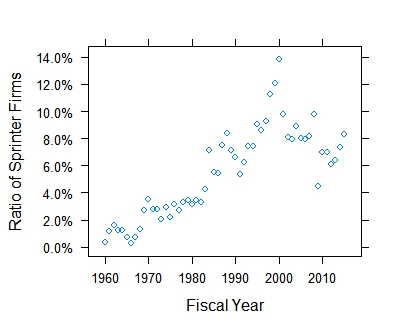
\includegraphics{CBFirms.jpeg}}}
    \caption{\label{fig:CBFirms}\textit{Evolution of the ratio of sprinter firms in the economy.}}
\end{figure}

\begin{figure}[!htbp]\centering \captionsetup{width=5.8in}
    \fbox{\resizebox{3.0in}{2.0in}{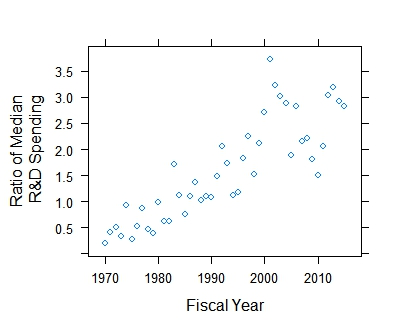
\includegraphics{RD_spending_ratio.jpeg}}}
    \caption{\label{fig:RD_spending_rat}\textit{Evolution of the ratio of median R\&D spending between sprinter firms and the whole economy.}}
\end{figure}

\begin{figure}[!htbp]\centering \captionsetup{width=5.8in}
    \fbox{\resizebox{3.0in}{2.0in}{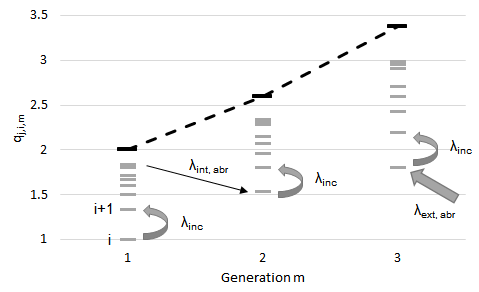
\includegraphics{QLadder.png}}}
    \caption{\label{fig:QLadder}\textit{Example of sequential innovations in a given product line, for different generations.}}
\end{figure}

\begin{table}[!htbp] \centering 
  \caption{Regression Results} 
  \label{tab:Pat_reg} 
\begin{tabular}{@{\extracolsep{5pt}}lD{.}{.}{-3} D{.}{.}{-3} D{.}{.}{-3} } 
\\[-1.8ex]\hline 
\hline \\[-1.8ex] 
 & \multicolumn{3}{c}{\textit{Dependent variable:}} \\ 
\cline{2-4} 
\\[-1.8ex] & \multicolumn{3}{c}{Labor Productivity} \\ 
\\[-1.8ex] & \multicolumn{1}{c}{(1)} & \multicolumn{1}{c}{(2)} & \multicolumn{1}{c}{(3)}\\ 
\hline \\[-1.8ex] 
 Dummy.t & 0.005 & 0.005 & 0.005 \\ 
  & (0.011) & (0.012) & (0.012) \\ 
  Dummy.t-1 & -0.012 & -0.013 & -0.013 \\ 
  & (0.012) & (0.012) & (0.012) \\ 
  Dummy.t-2 & 0.025^{*} & 0.022 & 0.022 \\ 
  & (0.012) & (0.012) & (0.012) \\ 
  Dummy.t-3 & 0.024^{*} & 0.021 & 0.020 \\ 
  & (0.012) & (0.012) & (0.012) \\ 
  Dummy.t-4 & -0.025^{*} & -0.030^{*} & -0.031^{*} \\ 
  & (0.012) & (0.012) & (0.012) \\ 
  Dummy.t-5 &  & 0.028^{*} & 0.026^{*} \\ 
  &  & (0.012) & (0.012) \\ 
  Dummy.t-6 &  &  & 0.013 \\ 
  &  &  & (0.013) \\ 
 \hline \\[-1.8ex] 
Firm fixed effects & Yes & Yes & Yes \\ 
Year fixed effects & Yes & Yes & Yes \\ 
Observations & \multicolumn{1}{c}{38,035} & \multicolumn{1}{c}{37,549} & \multicolumn{1}{c}{37,017} \\ 
R$^{2}$ & \multicolumn{1}{c}{0.0004} & \multicolumn{1}{c}{0.001} & \multicolumn{1}{c}{0.001} \\ 
\hline 
\hline \\[-1.8ex] 
\textit{Note:}  & \multicolumn{3}{r}{$^{*}$p$<$0.05; $^{**}$p$<$0.01; $^{***}$p$<$0.001} \\ 
\end{tabular} 
\end{table}

\begin{figure}[htb]\centering \captionsetup{width=5.8in}
    \fbox{\resizebox{3.0in}{2.0in}{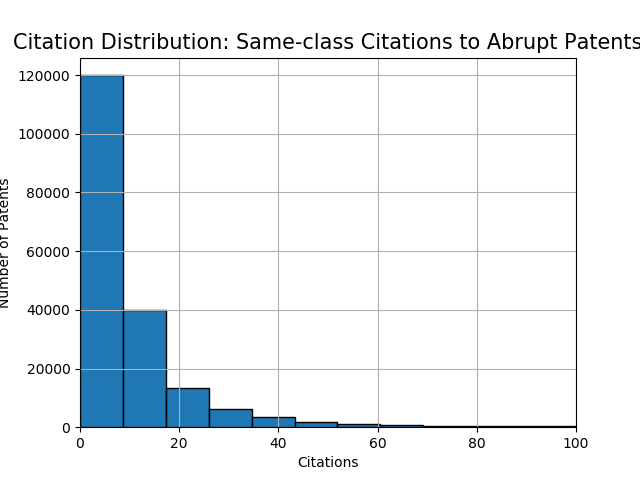
\includegraphics{SameClass_hist.png}}}
    \caption{\label{fig:SameClassDistr}\textit{Distribution of same-class abrupt patents by the number of received citations.}}
\end{figure}

\begin{figure}[htb]\centering \captionsetup{width=5.8in}
    \fbox{\resizebox{3.0in}{2.0in}{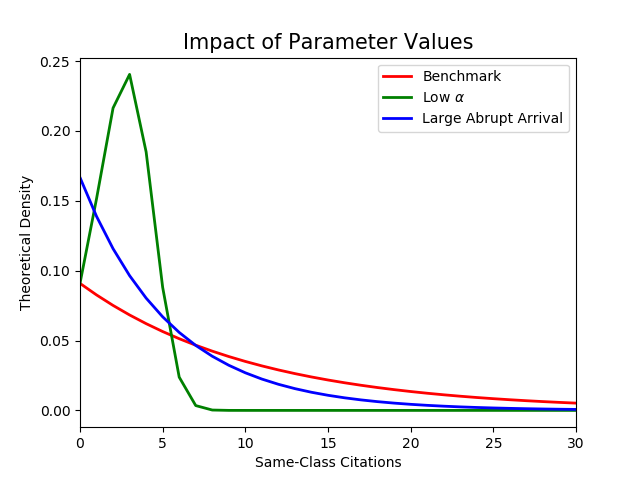
\includegraphics{Impact_parameters.png}}}
    \caption{\label{fig:ImpactPar}\textit{Theoretical distribution of patents per number of citations for different sets of parameters.}}
\end{figure}

\begin{figure}[htb]\centering \captionsetup{width=5.8in}
    \fbox{\resizebox{3.0in}{2.0in}{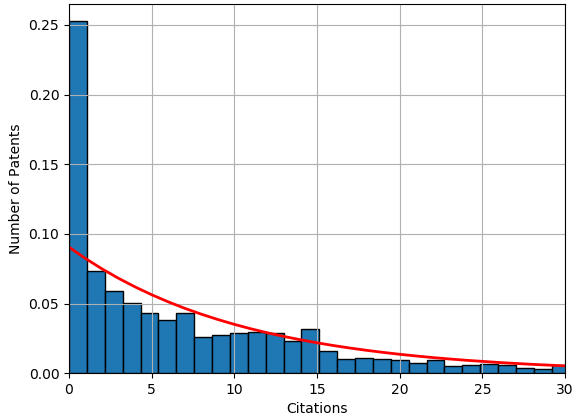
\includegraphics{MLE.png}}}
    \caption{\label{fig:MLE}\textit{Maximum likelihood estimated curve plotted over the same-class citation distribution.}}
\end{figure}

\begin{figure}[htb]\centering \captionsetup{width=5.8in}
    \fbox{\resizebox{3.0in}{2.0in}{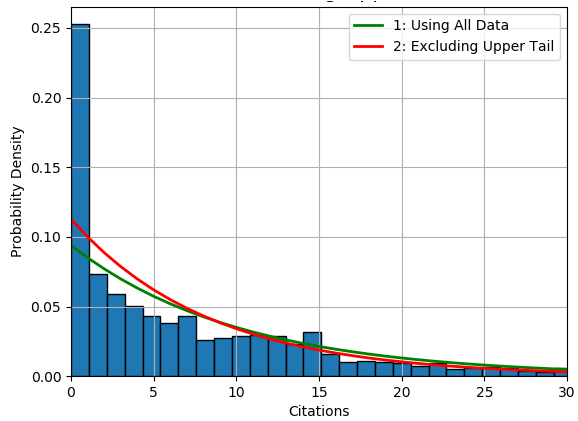
\includegraphics{MLE_extail.png}}}
    \caption{\label{fig:MLE_extail}\textit{Maximum likelihood estimated curves using the entire distribution or excluding the upper-tail.}}
\end{figure}

\begin{figure}[htb]\centering \captionsetup{width=5.8in}
    \fbox{\resizebox{3.0in}{2.0in}{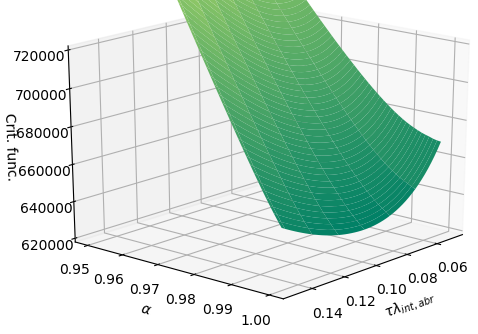
\includegraphics{Crit.png}}}
    \caption{\label{fig:Crit}\textit{3D plot of the criterion function of the maximum likelihood estimation for values of $\alpha$ and $\frac{\lambda_{abr, int} + \tau}{\lambda_{inc,0}}$.}}
\end{figure}

\begin{figure}[htb]\centering \captionsetup{width=5.8in}
    \fbox{\resizebox{3.0in}{2.0in}{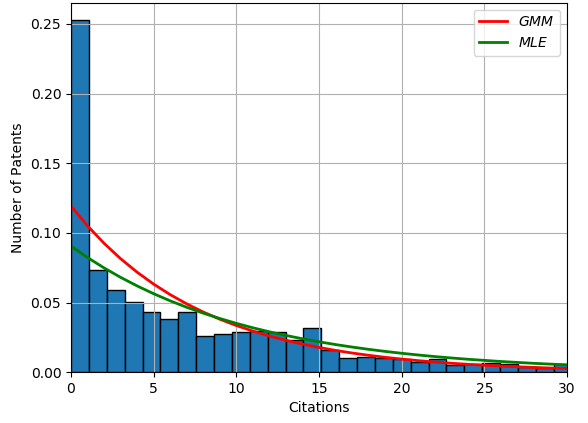
\includegraphics{GMM_MLE.png}}}
    \caption{\label{fig:GMM_MLE}\textit{Citation distribution for same-class abrupt patents and estimation results for MLE and GMM.}}
\end{figure}

\end{document}
